\section{Esempio di Istogramma}

Di seguito è riportato un semplice esempio di istogramma generato con Python e Matplotlib.

\begin{figure}[h!]
    \centering
    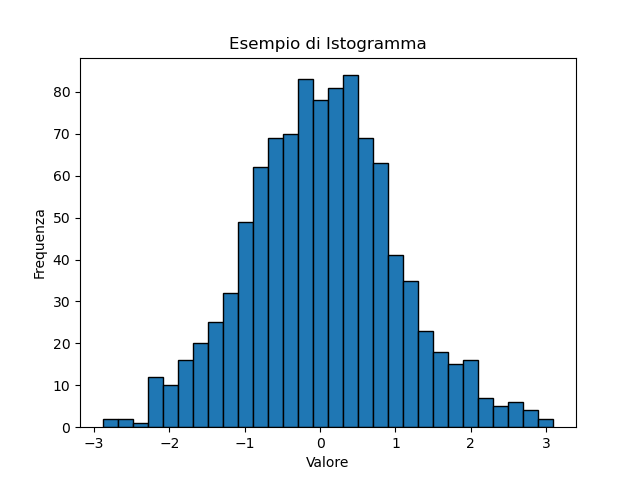
\includegraphics[width=0.8\textwidth]{histogram_example.png}
    \caption{Esempio di istogramma generato con Python e Matplotlib}
    \label{fig:histogram_example}
\end{figure}

\subsection{Codice Python per Generare l'Istogramma}

\begin{lstlisting}[language=Python, caption=Codice Python per generare un istogramma, label=code:histogram]
import matplotlib.pyplot as plt
import numpy as np

# Generazione di dati casuali
data = np.random.randn(1000)

# Creazione dell'istogramma
plt.hist(data, bins=30, edgecolor='black')

# Aggiunta di titolo e etichette
plt.title('Esempio di Istogramma')
plt.xlabel('Valore')
plt.ylabel('Frequenza')

# Salvataggio dell'istogramma
plt.savefig('histogram_example.png')
#se vuoi scaricare il file da google colab decommenta le righe:
#from google.colab import files
#files.download('histogram_example.png')
plt.show()
\end{lstlisting}

Nel codice sopra, abbiamo generato 1000 dati casuali con una distribuzione normale usando \texttt{numpy}. Questi dati sono stati suddivisi in 30 \textit{bins} per creare l'istogramma. Il parametro \texttt{edgecolor='black'} è utilizzato per disegnare i bordi neri intorno ai rettangoli dell'istogramma, rendendoli più chiari.






\subsection{La Curva di Gauss}

La distribuzione gaussiana è caratterizzata dalla seguente funzione densità di probabilità (pdf):

\begin{equation}
f(x|\mu,\sigma) = \frac{1}{\sigma \sqrt{2\pi}} e^{-\frac{(x-\mu)^2}{2\sigma^2}}
\end{equation}

dove:
\begin{itemize}
    \item $\mu$ è la media della distribuzione, che indica il valore centrale attorno al quale i dati sono distribuiti.
    \item $\sigma$ è la deviazione standard, che misura la dispersione dei dati rispetto alla media.
\end{itemize}

La curva di Gauss ha una forma a campana, simmetrica rispetto alla media $\mu$. La maggior parte dei dati (circa il 68\%) si trova entro un intervallo di una deviazione standard dalla media ($\mu \pm \sigma$), mentre il 95\% dei dati si trova entro due deviazioni standard ($\mu \pm 2\sigma$). Questo comportamento rende la distribuzione gaussiana particolarmente utile per descrivere fenomeni naturali dove le variazioni sono dovute a molti fattori piccoli e indipendenti. In figura \ref{fig:curva_gaussiana} vediamo il tipico aspetto di una gaussiana.

\begin{figure}[h!]
    \centering
     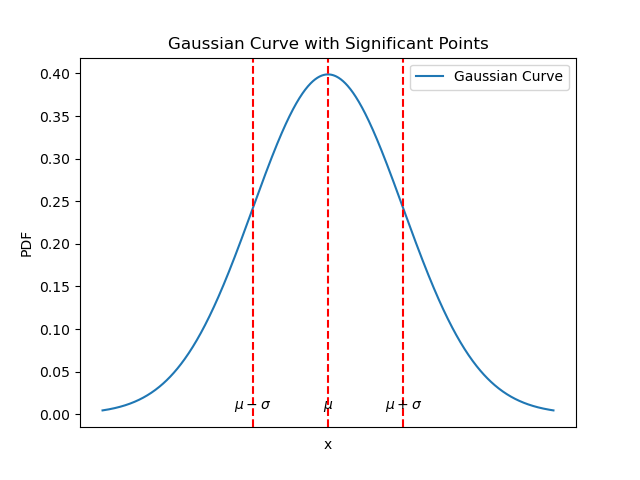
\includegraphics[scale=0.7]{curva_gaussiana.png} 
    \caption{Curva Gaussiana con Evidenziati \(\overline{\mu}\), \(\overline{\mu} - \sigma\), e \(\overline{\mu} + \sigma\)}
    \label{fig:curva_gaussiana}
\end{figure}


